\documentclass[sigconf]{acmart}


\usepackage{hyperref}

%\usepackage{endfloat}
%\renewcommand{\efloatseparator}{\mbox{}} % no new page between figures

\usepackage{booktabs} % For formal tables

\settopmatter{printacmref=false} % Removes citation information below abstract
\renewcommand\footnotetextcopyrightpermission[1]{} % removes footnote with conference information in first column
\pagestyle{plain} % removes running headers


\begin{document}
\title{Big Data Analytics in Weather Forecasting}


\author{Himani Bhatt}
\affiliation{%
  \institution{Indiana University}
  \city{Bloomington} 
  \state{Indiana} 
}
\email{himbhatt@iu.edu}



% The default list of authors is too long for headers}
\renewcommand{\shortauthors}{H. Bhatt}



\begin{abstract}

Big data analytics applications help data scientists, statisticians to analyze tons of data in order to have useful insights and make predictions based on it. In majority of the cases the data that has been dealt with is unstructured and complex. In case of weather forecasting, data about the current state of atmosphere (that includes wind, humidity, temperature etc) is gathered, and by using concepts of meteorology, the evolution of atmosphere in future is predicted.

\end{abstract}

\keywords{ HID $202$, i$523$, NWP(Numerical Weather Predictions), Supercomputers.}

\maketitle

\section{Introduction} 

Daily over 20 terabytes of data get generated of different key weather-related parameters like wind speeds, temperature readings, satellite images, barometric pressure from different locations. Yet the extreme weather events cause huge amount of loss and damage worldwide. For instance, 90 percent of the crop losses are due to weather calamities all over the world. The ability to better predict the weather could slash this by up to 25 percent. The ability to use the big data generated efficiently directly affects the chances to reduce economic loss, environmental damage and fatality. This can be considered as the best motivation to improve and invest in this extremely challenging task.Weather forecasting is considered extremely challenging since large number of variables are involved and their interaction is also very complex.
The data accumulation is done from the sources like trained observers, weather balloons, weather stations, satellites, radar, etc. The data is then plugged into super computers which uses numerical forecast equations to create forecast models of the atmosphere and to produce the meteorological analysis.
\cite{Youtube}.

\section{History of Weather Prediction}


After the invention of the first electronic computer ENIAC, a group of meteorologists at New Jersey's institute for Advanced Study produced first weather forecast using ENIAC and numeric prediction techniques back in 1950. There forecast was for 24 hours but they took more than 24 hours to complete. This can be marked as the need for the beginning of numerical weather predictions \cite{History01}.
\\

\subsection*{Numerical weather prediction models}


Any typical numeric weather prediction model will have complex and multidimensional data. These models divide earth into various atmospheric boxes. For each box they try to apply mathematical equations for the current weather and they try to forecast weather for coming days. These equations are derived from physics and fluid motion. This data is divided horizontally as latitude longitude and vertically as different pressure levels. And hence it is multidimensional.\\

The higher the resolution of the data, more is the accuracy of the NWP models. Because of improved resolution, improved data sources, and improved physics processes, enormous advancements  are seen in the atmospheric modelling techniques. With the models improving, requirement of high computing powers increase proportionally, and the models now need supercomputers to run operationally.\\


\begin{figure}
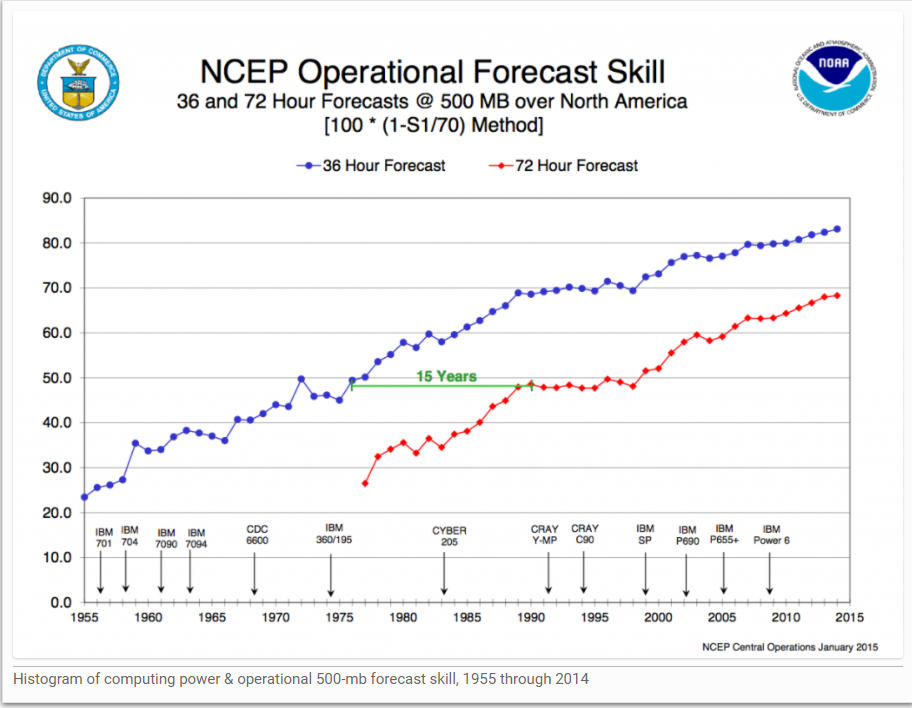
\includegraphics{images/Big data image.PNG}
\caption{Histogram by NCEP(National Centres for Environmental Prediction) showing trends in computing power and operational model skill over time \cite{History01}.}
\end{figure}


\section{Weather Prediction in Modern times}

A company named Weather Analytics has been forecasting a week's weather in advance by analyzing US Government's weather service data of past 38 years. It's methodology includes placing global data in a 35km by 35km grid and then extraction of relevant variables from the generated outputs which are often in range of 650,000 per hour.\\

The company says: ``We then extract pertinent variables and create/calculate numerous others. We store this massive amount of weather information in databases which allows us to: present the data quickly, calculate additional variables, and uniquely package the data'' \cite{Zdnet}.\\

Enhancement of data processing power is clearly exemplified by the supercomputer at UK based firm called Met Office, which has 480,000 cores, two million GB of memory and 17,000TB of storage. This 140 tonnes processing giant is capable of performing over 23,000 trillion operations per second, which has brought the accuracy of modern 4 days forecasts on par with that of 1 day forecasts 30 years ago through improved data model resolution and enabling usage of smaller grid sizes \cite{Zdnet}.

\section{Hadoop for climate Analytics}

The NASA center for climate simulation uses Apache Hadoop for performing high performance computing as it combines distributed storage of large data sets with parallel computing and optimizes computer clusters. It has built a new platform with Hadoop for developing new analysis capabilities. Hadoop Bloom filter is utilized that helps to identify rapidly and memory efficiently if an element is present.\\


\subsection*{Advantage of using HDFS and MapReduce}

Hadoop is resilient to failure, provide load balancing and parallelization. When the data is sent to an individual node, it is also sent to other nodes in the cluster. So in case of failure their will be a copy of data available.Storage nodes and compute nodes are same. It means that tools for the data processing are on the same servers where the data is located, which result in fast data processing. Hadoop is capable of processing terabytes of unstructured data in just minutes and petabytes in hours. Thus is highly used in weather analytics.The requested operations are mapped to the appropriate nodes using specified key \cite{Hadoop01}. \\

\section{Current Weather Forecasting Models}



\subsection{Deep Thunder'-  World's Most Advanced Hyper-Local Weather Forecasting Model}


Deep thunder is a research project by IBM and it is headed by Lloyd Treinish. The scientists in IBM developed first parallel processing supercomputers that can be used for weather modeling. This supercomputer is based on IBM RS/6000 SP( it is a family of Reduced instruction set computer based on UNIX servers, supercomputers made by IBM in 1990's). It was first installed at National Weather Service office in Georgia in 1966.\\
With high accuracy deep thunder can deliver hyper localized weather conditions up to three days in advance, with calculations as fine as every mile and as granular as every 10 minutes. Deep thunder can forecast weather for an 84 hours duration.Rio De Janeiro's city operation center is already using Deep Thunder \cite{Coclus01}.


\begin{figure}
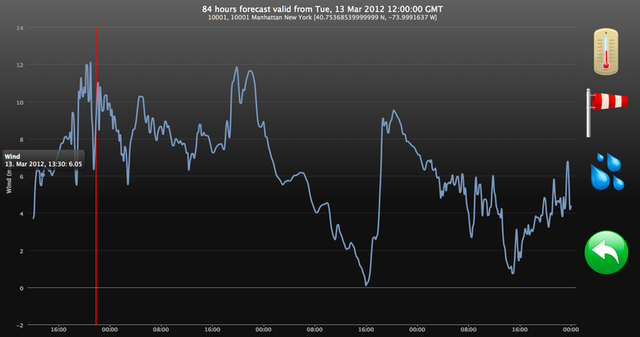
\includegraphics{images/Deep thunder.png}
\caption{84 hours forecast by predicted by Deep Thunder \cite{Image}.}
\end{figure}

Deep thunder uses a 3D telescopic grid where data from one model is fed into another model, that is called coupled models in climatology. This data is then verified with the historical data. They work in collaboration with National Oceanic and Atmospheric Administration(NOAA), and use global models provided by them. In order to decrease the amount of processing required, they zoom in, that exponentially increase the resolution, down to models with resolution as small as 1 meter. This layered model approach shrinks big high performance computing problem to a relatively smaller footprint of parallel processing systems. The data sources of Deep Thunder are public satellite sources, underground personal weather stations, smart phone barometer etc.  \cite{Deep01}.


\subsection{Hybrid renewable energy forecasting(HyRef)}


Together with focusing on the damages done by weather we can also work on creating renewable resources. Wind and solar energy can be used to produce enormous amount of power. Forecasting the wind and solar availability will help in reducing the uncertainty associated with variable renewable energy generation.
Hyref combines big data analytics and weather modeling technology to accurately forecast the availability of wind power and solar energy. This helps the  energy providers to optimize the output and integrate more renewable energy into the power grid \cite{Hyref02}.\\

Hyref has the following key components :\\

\begin{description}

\item [$\bullet$ Weather modeling capabilities]- The modeling is done at very granular level, from a square kilometer to vertical dimensions like heights where rotors and turbine hubs are located.

\item [$\bullet$ Advanced imaging technology]- Cloud imaging, advanced cameras.

\item [$\bullet$ Sensors on the turbines]- Highly perceptive sensors are used to monitor the turbulence, temperature and direction of wind.

\item [$\bullet$ Analytical capabilities]- Hyref use cloud image analytics and advanced numerical prediction models to calculate weather impacts on solar generation and to forecast cloud movements. SAS is used for this purpose and it is on DB2 platform \cite{Hyref04}.\\

\end{description}


``Applying analytics and harnessing big data will allow utilities to tackle the intermittent nature of renewable energy and forecast power production from solar and wind, in a way that has never been done before,'' said Brad Gammons, general manager of IBM's Global Energy and Utilities Industry group, in a statement. ``We have developed an intelligent system that combines weather and power forecasting to increase system availability and optimize power grid performance'' \cite{Hyref03}.


\section{Conclusion}


Ability to better predict the weather can have a dramatic impact on our planet by creating new energy resources and helps us to be better prepared for weather related incidents across all industries. Businesses from retail, production, energy, agriculture, water resource management are all using predictions from weather models to make decisions. Thus a better weather forecast will definitely have a positive economic impact. Not only economic impact, it can potentially save thousands of lives and safeguard property in times to come.\\

Increasing evidence of climate change worldwide is prompting governments and scientists to take action to protect people and property from its effects. One such instance is the up-gradation of national weather information system  by South Korea, after being hit by Typhoon Sanba and Hwangsa storms. The upgrade has increased agency's data capacity drastically. And it has now become Korea's most capable storage system. The output comes as the better understanding of the weather patterns and predicting the ferocity and location of the weather events.This project of South Korea dramatically illustrates today's big data phenomenon and its impact on weather forecasting.\\

\begin{acks}
The author would like to thank Dr. Gregor von Laszewski and the Assistant Instructors for their feedback and help.
\end{acks}



\bibliographystyle{ACM-Reference-Format}
\bibliography{report} 

\end{document}
